% $Id$
%==============================================================================
\chapter{UML Component Design}
%==============================================================================

Remember, component based development starts with component design.
A component designer specifies components using the 
{\it Interface Definition Language} (IDL).

On the other side, the OMG proposes a {\it Model Driven Architecture} (MDA) 
where development starts at abstract levels called 
{\it Platform Independent Models} (PIM).
After some refinement steps, these PIM are transformed to 
{\it Platform Specific Models} (PSM).
Finally, from PSM, tools can generate source code that implements the modeled 
application.

OK, that's the vision. 
In practice, there are still problems in applying MDA because modeling of 
behavior is difficult (even in UML 1.x) and tool support is marginal. 
However, the MDA ideas are very interesting, thus CCM Tools make a first step 
in this direction by designing components in UML 1.4.

%------------------------------------------------------------------------------
\section{Model driven development}
%------------------------------------------------------------------------------

To design components in UML we use the {\it UML Profile for CCM} 
\cite{UML-CORBA-Profile,UML-CCM-Profile}. 
This profile is basically a class diagram using a bunch of stereotypes.
For each IDL construct there is a corresponding representation in UML class 
diagram.

\begin{figure}[htbp]
    \begin{center}
        \includegraphics [width=9cm,angle=0] {UMLComponentDesign}
        \caption{UML component design}
        \label{fig:uml-component-design}
    \end{center}
\end{figure}

A component designer paints the UML representation of components using a UML 
tool that stores diagrams in XMI 1.1 format 
(Fig.~\ref{fig:uml-component-design}).
Currently we use {\it MagicDraw} where a community edition can be downloaded 
for free).

From the stored XMI file, the {\tt uml2idl} generator creates a single IDL file.
Optionally, this IDL file can be validated and fragmented into many source files
(that are linked via include statements) by using the {\tt idl3} generator.
IDL file partitioning prevents a developer from redundant IDL definitions 
especially when processing more components at the same time.


%------------------------------------------------------------------------------
\section{The designer's job}
%------------------------------------------------------------------------------
To figure out the new tasks of a component designer, we present a concrete 
example.
Fig.~\ref{fig:uml-component-example} shows the UML representation of our first 
component definition.
The mapping from UML profile to IDL is straight forward. A UML 
package is mapped to an IDL module, UML classes are mapped to IDL constructs
corresponding to their given stereotypes (see Example \ref{example:Exceptions} 
to \ref{example:component}).
\begin{figure}[htbp]
    \begin{center}
        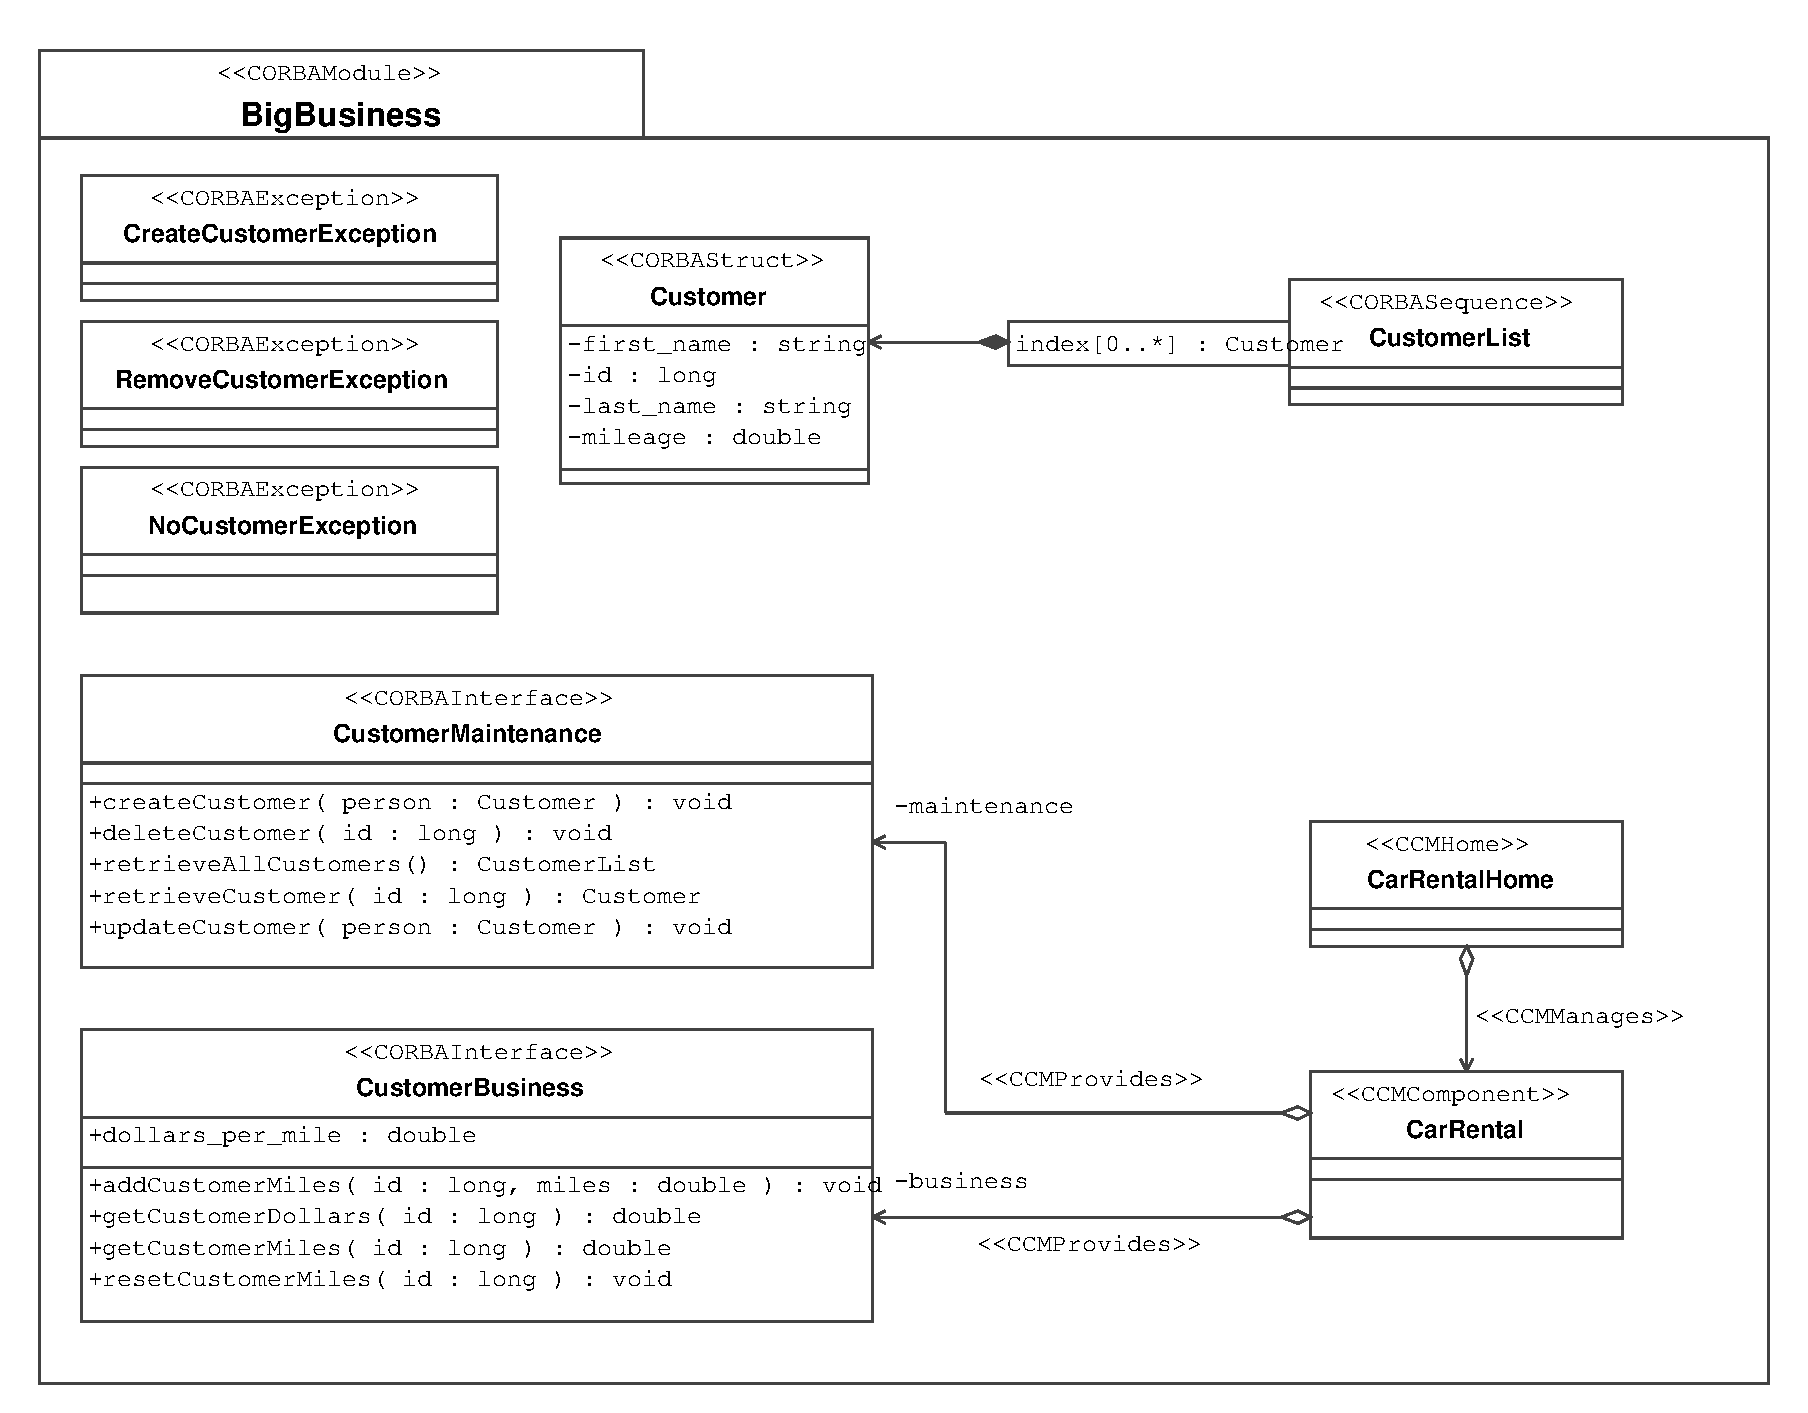
\includegraphics [width=13cm,angle=0] {uml/Example1}
        \caption{CarRental component in UML}
        \label{fig:uml-component-example}
    \end{center}
\end{figure}

We store the diagram (as an {\it XMI 1.1} file) in a directory called 
{\tt example2}, change to that directory and run the {\tt uml2idl} generator:
\begin{small}
\begin{verbatim}
    ~/example2> uml2idl uml/Example2.xml.zip example2
\end{verbatim}
\end{small}
After running {\tt uml2idl}, the new directory contains the following files:
\begin{small}
\begin{verbatim}
    example2/
    |-- example2.idl
    |-- example2.ocl
    `-- uml
        `-- Example2.xml.zip
\end{verbatim}
\end{small}

\newpage
\begin{itemize}
\item {\tt Example2.xml.zip}\\
This is the XMI file written from a UML tool.

\item {\tt example2.idl}\\ 
This file contains all generated IDL statements. 

\item {\tt example2.ocl} \\
In this file, all OCL expressions defined in the source model are stored.
Currently, we don't care about this file but we will use it in context of
Design by Contract. 
\end{itemize}

From the single IDL3 file, we generate a bunch of well structured 
IDL3 files as done with manually written files:
\begin{small}
\begin{verbatim}
    ~/example2> ccmtools-generate idl3 -o CarRental/idl3 *.idl
\end{verbatim}
\end{small}

Again, we have separated interfaces from component definitions:
\begin{small}
\begin{verbatim}
CarRental
`-- idl3
    |-- component
    |   `-- BigBusiness
    |       |-- CarRental.idl
    |       |-- CarRentalHome.idl
    |       |-- CarRentalHome_mirror.idl
    |       `-- CarRental_mirror.idl
    `-- interface
        `-- BigBusiness
            |-- CreateCustomerException.idl
            |-- Customer.idl
            |-- CustomerBusiness.idl
            |-- CustomerList.idl
            |-- CustomerMaintenance.idl
            |-- NoCustomerException.idl
            `-- RemoveCustomerException.idl
\end{verbatim}
\end{small}

That's it, we have made the first step toward MDA! 

But remember, we have only generated a component's structural description from
a UML diagram. The generated IDL file is a pure syntax description, without 
any semantics.  


%------------------------------------------------------------------------------
\section{The developers's job}
%------------------------------------------------------------------------------

It's important to know, that a developer's job does not change whether a 
component is designed in UML or IDL.
In both cases, a developer starts from the IDL3 file structure as shown above.
